% Options for packages loaded elsewhere
\PassOptionsToPackage{unicode}{hyperref}
\PassOptionsToPackage{hyphens}{url}
%
\documentclass[
]{article}
\usepackage{amsmath,amssymb}
\usepackage{lmodern}
\usepackage{iftex}
\ifPDFTeX
  \usepackage[T1]{fontenc}
  \usepackage[utf8]{inputenc}
  \usepackage{textcomp} % provide euro and other symbols
\else % if luatex or xetex
  \usepackage{unicode-math}
  \defaultfontfeatures{Scale=MatchLowercase}
  \defaultfontfeatures[\rmfamily]{Ligatures=TeX,Scale=1}
\fi
% Use upquote if available, for straight quotes in verbatim environments
\IfFileExists{upquote.sty}{\usepackage{upquote}}{}
\IfFileExists{microtype.sty}{% use microtype if available
  \usepackage[]{microtype}
  \UseMicrotypeSet[protrusion]{basicmath} % disable protrusion for tt fonts
}{}
\makeatletter
\@ifundefined{KOMAClassName}{% if non-KOMA class
  \IfFileExists{parskip.sty}{%
    \usepackage{parskip}
  }{% else
    \setlength{\parindent}{0pt}
    \setlength{\parskip}{6pt plus 2pt minus 1pt}}
}{% if KOMA class
  \KOMAoptions{parskip=half}}
\makeatother
\usepackage{xcolor}
\IfFileExists{xurl.sty}{\usepackage{xurl}}{} % add URL line breaks if available
\IfFileExists{bookmark.sty}{\usepackage{bookmark}}{\usepackage{hyperref}}
\hypersetup{
  pdftitle={RNA-seq Data Analysis Pipeline},
  pdfauthor={Md Musaddaqul Hasib},
  hidelinks,
  pdfcreator={LaTeX via pandoc}}
\urlstyle{same} % disable monospaced font for URLs
\usepackage[margin=1in]{geometry}
\usepackage{color}
\usepackage{fancyvrb}
\newcommand{\VerbBar}{|}
\newcommand{\VERB}{\Verb[commandchars=\\\{\}]}
\DefineVerbatimEnvironment{Highlighting}{Verbatim}{commandchars=\\\{\}}
% Add ',fontsize=\small' for more characters per line
\usepackage{framed}
\definecolor{shadecolor}{RGB}{248,248,248}
\newenvironment{Shaded}{\begin{snugshade}}{\end{snugshade}}
\newcommand{\AlertTok}[1]{\textcolor[rgb]{0.94,0.16,0.16}{#1}}
\newcommand{\AnnotationTok}[1]{\textcolor[rgb]{0.56,0.35,0.01}{\textbf{\textit{#1}}}}
\newcommand{\AttributeTok}[1]{\textcolor[rgb]{0.77,0.63,0.00}{#1}}
\newcommand{\BaseNTok}[1]{\textcolor[rgb]{0.00,0.00,0.81}{#1}}
\newcommand{\BuiltInTok}[1]{#1}
\newcommand{\CharTok}[1]{\textcolor[rgb]{0.31,0.60,0.02}{#1}}
\newcommand{\CommentTok}[1]{\textcolor[rgb]{0.56,0.35,0.01}{\textit{#1}}}
\newcommand{\CommentVarTok}[1]{\textcolor[rgb]{0.56,0.35,0.01}{\textbf{\textit{#1}}}}
\newcommand{\ConstantTok}[1]{\textcolor[rgb]{0.00,0.00,0.00}{#1}}
\newcommand{\ControlFlowTok}[1]{\textcolor[rgb]{0.13,0.29,0.53}{\textbf{#1}}}
\newcommand{\DataTypeTok}[1]{\textcolor[rgb]{0.13,0.29,0.53}{#1}}
\newcommand{\DecValTok}[1]{\textcolor[rgb]{0.00,0.00,0.81}{#1}}
\newcommand{\DocumentationTok}[1]{\textcolor[rgb]{0.56,0.35,0.01}{\textbf{\textit{#1}}}}
\newcommand{\ErrorTok}[1]{\textcolor[rgb]{0.64,0.00,0.00}{\textbf{#1}}}
\newcommand{\ExtensionTok}[1]{#1}
\newcommand{\FloatTok}[1]{\textcolor[rgb]{0.00,0.00,0.81}{#1}}
\newcommand{\FunctionTok}[1]{\textcolor[rgb]{0.00,0.00,0.00}{#1}}
\newcommand{\ImportTok}[1]{#1}
\newcommand{\InformationTok}[1]{\textcolor[rgb]{0.56,0.35,0.01}{\textbf{\textit{#1}}}}
\newcommand{\KeywordTok}[1]{\textcolor[rgb]{0.13,0.29,0.53}{\textbf{#1}}}
\newcommand{\NormalTok}[1]{#1}
\newcommand{\OperatorTok}[1]{\textcolor[rgb]{0.81,0.36,0.00}{\textbf{#1}}}
\newcommand{\OtherTok}[1]{\textcolor[rgb]{0.56,0.35,0.01}{#1}}
\newcommand{\PreprocessorTok}[1]{\textcolor[rgb]{0.56,0.35,0.01}{\textit{#1}}}
\newcommand{\RegionMarkerTok}[1]{#1}
\newcommand{\SpecialCharTok}[1]{\textcolor[rgb]{0.00,0.00,0.00}{#1}}
\newcommand{\SpecialStringTok}[1]{\textcolor[rgb]{0.31,0.60,0.02}{#1}}
\newcommand{\StringTok}[1]{\textcolor[rgb]{0.31,0.60,0.02}{#1}}
\newcommand{\VariableTok}[1]{\textcolor[rgb]{0.00,0.00,0.00}{#1}}
\newcommand{\VerbatimStringTok}[1]{\textcolor[rgb]{0.31,0.60,0.02}{#1}}
\newcommand{\WarningTok}[1]{\textcolor[rgb]{0.56,0.35,0.01}{\textbf{\textit{#1}}}}
\usepackage{graphicx}
\makeatletter
\def\maxwidth{\ifdim\Gin@nat@width>\linewidth\linewidth\else\Gin@nat@width\fi}
\def\maxheight{\ifdim\Gin@nat@height>\textheight\textheight\else\Gin@nat@height\fi}
\makeatother
% Scale images if necessary, so that they will not overflow the page
% margins by default, and it is still possible to overwrite the defaults
% using explicit options in \includegraphics[width, height, ...]{}
\setkeys{Gin}{width=\maxwidth,height=\maxheight,keepaspectratio}
% Set default figure placement to htbp
\makeatletter
\def\fps@figure{htbp}
\makeatother
\setlength{\emergencystretch}{3em} % prevent overfull lines
\providecommand{\tightlist}{%
  \setlength{\itemsep}{0pt}\setlength{\parskip}{0pt}}
\setcounter{secnumdepth}{-\maxdimen} % remove section numbering
\ifLuaTeX
  \usepackage{selnolig}  % disable illegal ligatures
\fi

\title{RNA-seq Data Analysis Pipeline}
\author{Md Musaddaqul Hasib}
\date{2022-12-23}

\begin{document}
\maketitle

\hypertarget{loading-packages}{%
\subsection{Loading Packages}\label{loading-packages}}

\begin{Shaded}
\begin{Highlighting}[]
\FunctionTok{library}\NormalTok{(org.Mm.eg.db)}
\end{Highlighting}
\end{Shaded}

\begin{verbatim}
## Loading required package: AnnotationDbi
\end{verbatim}

\begin{verbatim}
## Loading required package: stats4
\end{verbatim}

\begin{verbatim}
## Loading required package: BiocGenerics
\end{verbatim}

\begin{verbatim}
## 
## Attaching package: 'BiocGenerics'
\end{verbatim}

\begin{verbatim}
## The following objects are masked from 'package:stats':
## 
##     IQR, mad, sd, var, xtabs
\end{verbatim}

\begin{verbatim}
## The following objects are masked from 'package:base':
## 
##     anyDuplicated, append, as.data.frame, basename, cbind, colnames,
##     dirname, do.call, duplicated, eval, evalq, Filter, Find, get, grep,
##     grepl, intersect, is.unsorted, lapply, Map, mapply, match, mget,
##     order, paste, pmax, pmax.int, pmin, pmin.int, Position, rank,
##     rbind, Reduce, rownames, sapply, setdiff, sort, table, tapply,
##     union, unique, unsplit, which.max, which.min
\end{verbatim}

\begin{verbatim}
## Loading required package: Biobase
\end{verbatim}

\begin{verbatim}
## Welcome to Bioconductor
## 
##     Vignettes contain introductory material; view with
##     'browseVignettes()'. To cite Bioconductor, see
##     'citation("Biobase")', and for packages 'citation("pkgname")'.
\end{verbatim}

\begin{verbatim}
## Loading required package: IRanges
\end{verbatim}

\begin{verbatim}
## Loading required package: S4Vectors
\end{verbatim}

\begin{verbatim}
## 
## Attaching package: 'S4Vectors'
\end{verbatim}

\begin{verbatim}
## The following objects are masked from 'package:base':
## 
##     expand.grid, I, unname
\end{verbatim}

\begin{verbatim}
## 
\end{verbatim}

\begin{Shaded}
\begin{Highlighting}[]
\FunctionTok{library}\NormalTok{(}\StringTok{"DESeq2"}\NormalTok{)}
\end{Highlighting}
\end{Shaded}

\begin{verbatim}
## Loading required package: GenomicRanges
\end{verbatim}

\begin{verbatim}
## Loading required package: GenomeInfoDb
\end{verbatim}

\begin{verbatim}
## Loading required package: SummarizedExperiment
\end{verbatim}

\begin{verbatim}
## Loading required package: MatrixGenerics
\end{verbatim}

\begin{verbatim}
## Loading required package: matrixStats
\end{verbatim}

\begin{verbatim}
## 
## Attaching package: 'matrixStats'
\end{verbatim}

\begin{verbatim}
## The following objects are masked from 'package:Biobase':
## 
##     anyMissing, rowMedians
\end{verbatim}

\begin{verbatim}
## 
## Attaching package: 'MatrixGenerics'
\end{verbatim}

\begin{verbatim}
## The following objects are masked from 'package:matrixStats':
## 
##     colAlls, colAnyNAs, colAnys, colAvgsPerRowSet, colCollapse,
##     colCounts, colCummaxs, colCummins, colCumprods, colCumsums,
##     colDiffs, colIQRDiffs, colIQRs, colLogSumExps, colMadDiffs,
##     colMads, colMaxs, colMeans2, colMedians, colMins, colOrderStats,
##     colProds, colQuantiles, colRanges, colRanks, colSdDiffs, colSds,
##     colSums2, colTabulates, colVarDiffs, colVars, colWeightedMads,
##     colWeightedMeans, colWeightedMedians, colWeightedSds,
##     colWeightedVars, rowAlls, rowAnyNAs, rowAnys, rowAvgsPerColSet,
##     rowCollapse, rowCounts, rowCummaxs, rowCummins, rowCumprods,
##     rowCumsums, rowDiffs, rowIQRDiffs, rowIQRs, rowLogSumExps,
##     rowMadDiffs, rowMads, rowMaxs, rowMeans2, rowMedians, rowMins,
##     rowOrderStats, rowProds, rowQuantiles, rowRanges, rowRanks,
##     rowSdDiffs, rowSds, rowSums2, rowTabulates, rowVarDiffs, rowVars,
##     rowWeightedMads, rowWeightedMeans, rowWeightedMedians,
##     rowWeightedSds, rowWeightedVars
\end{verbatim}

\begin{verbatim}
## The following object is masked from 'package:Biobase':
## 
##     rowMedians
\end{verbatim}

\begin{Shaded}
\begin{Highlighting}[]
\FunctionTok{library}\NormalTok{(}\StringTok{"genefilter"}\NormalTok{)}
\end{Highlighting}
\end{Shaded}

\begin{verbatim}
## 
## Attaching package: 'genefilter'
\end{verbatim}

\begin{verbatim}
## The following objects are masked from 'package:MatrixGenerics':
## 
##     rowSds, rowVars
\end{verbatim}

\begin{verbatim}
## The following objects are masked from 'package:matrixStats':
## 
##     rowSds, rowVars
\end{verbatim}

\begin{Shaded}
\begin{Highlighting}[]
\FunctionTok{library}\NormalTok{(ggrepel)}
\end{Highlighting}
\end{Shaded}

\begin{verbatim}
## Loading required package: ggplot2
\end{verbatim}

\begin{Shaded}
\begin{Highlighting}[]
\FunctionTok{library}\NormalTok{(data.table)}
\end{Highlighting}
\end{Shaded}

\begin{verbatim}
## 
## Attaching package: 'data.table'
\end{verbatim}

\begin{verbatim}
## The following object is masked from 'package:SummarizedExperiment':
## 
##     shift
\end{verbatim}

\begin{verbatim}
## The following object is masked from 'package:GenomicRanges':
## 
##     shift
\end{verbatim}

\begin{verbatim}
## The following object is masked from 'package:IRanges':
## 
##     shift
\end{verbatim}

\begin{verbatim}
## The following objects are masked from 'package:S4Vectors':
## 
##     first, second
\end{verbatim}

\begin{Shaded}
\begin{Highlighting}[]
\FunctionTok{library}\NormalTok{(}\StringTok{"dplyr"}\NormalTok{)}
\end{Highlighting}
\end{Shaded}

\begin{verbatim}
## 
## Attaching package: 'dplyr'
\end{verbatim}

\begin{verbatim}
## The following objects are masked from 'package:data.table':
## 
##     between, first, last
\end{verbatim}

\begin{verbatim}
## The following object is masked from 'package:matrixStats':
## 
##     count
\end{verbatim}

\begin{verbatim}
## The following objects are masked from 'package:GenomicRanges':
## 
##     intersect, setdiff, union
\end{verbatim}

\begin{verbatim}
## The following object is masked from 'package:GenomeInfoDb':
## 
##     intersect
\end{verbatim}

\begin{verbatim}
## The following object is masked from 'package:AnnotationDbi':
## 
##     select
\end{verbatim}

\begin{verbatim}
## The following objects are masked from 'package:IRanges':
## 
##     collapse, desc, intersect, setdiff, slice, union
\end{verbatim}

\begin{verbatim}
## The following objects are masked from 'package:S4Vectors':
## 
##     first, intersect, rename, setdiff, setequal, union
\end{verbatim}

\begin{verbatim}
## The following object is masked from 'package:Biobase':
## 
##     combine
\end{verbatim}

\begin{verbatim}
## The following objects are masked from 'package:BiocGenerics':
## 
##     combine, intersect, setdiff, union
\end{verbatim}

\begin{verbatim}
## The following objects are masked from 'package:stats':
## 
##     filter, lag
\end{verbatim}

\begin{verbatim}
## The following objects are masked from 'package:base':
## 
##     intersect, setdiff, setequal, union
\end{verbatim}

\begin{Shaded}
\begin{Highlighting}[]
\FunctionTok{library}\NormalTok{(}\StringTok{"ggplot2"}\NormalTok{)}
\end{Highlighting}
\end{Shaded}

\hypertarget{data-directory}{%
\subsection{Data directory}\label{data-directory}}

\begin{Shaded}
\begin{Highlighting}[]
\NormalTok{data }\OtherTok{\textless{}{-}} \FunctionTok{load}\NormalTok{(}\StringTok{\textquotesingle{}/ihome/yufeihuang/zhl169/timothy/Gao\_mouse\_CASTOR1/feature\_counts.RData\textquotesingle{}}\NormalTok{)}
\end{Highlighting}
\end{Shaded}

\hypertarget{loading-dataset}{%
\subsection{Loading Dataset}\label{loading-dataset}}

\begin{Shaded}
\begin{Highlighting}[]
\NormalTok{counts\_KO }\OtherTok{\textless{}{-}}\NormalTok{ count\_matrix\_KO}\SpecialCharTok{$}\NormalTok{counts}
\NormalTok{counts\_WT }\OtherTok{\textless{}{-}}\NormalTok{ count\_matrix\_WT}\SpecialCharTok{$}\NormalTok{counts}
\NormalTok{count\_matrix }\OtherTok{\textless{}{-}} \FunctionTok{cbind}\NormalTok{(counts\_KO, counts\_WT)}
\end{Highlighting}
\end{Shaded}

\hypertarget{what-is-in-count-matrix}{%
\subsection{What is in count matrix?}\label{what-is-in-count-matrix}}

\begin{Shaded}
\begin{Highlighting}[]
\FunctionTok{dim}\NormalTok{(count\_matrix)}
\end{Highlighting}
\end{Shaded}

\begin{verbatim}
## [1] 55414    48
\end{verbatim}

\begin{Shaded}
\begin{Highlighting}[]
\FunctionTok{head}\NormalTok{(}\FunctionTok{rownames}\NormalTok{(count\_matrix))}
\end{Highlighting}
\end{Shaded}

\begin{verbatim}
## [1] "ENSMUSG00000102693.2" "ENSMUSG00000064842.3" "ENSMUSG00000051951.6"
## [4] "ENSMUSG00000102851.2" "ENSMUSG00000103377.2" "ENSMUSG00000104017.2"
\end{verbatim}

\begin{Shaded}
\begin{Highlighting}[]
\FunctionTok{head}\NormalTok{(}\FunctionTok{colnames}\NormalTok{(count\_matrix))}
\end{Highlighting}
\end{Shaded}

\begin{verbatim}
## [1] "C1-KO1-0_S7.sorted.bam"          "C1-KO1-LPS-12hr_S12.sorted.bam" 
## [3] "C1-KO1-LPS-1hr_S9.sorted.bam"    "C1-KO1-LPS-2hr_S10.sorted.bam"  
## [5] "C1-KO1-LPS-6hr_S11.sorted.bam"   "C1-KO1-LPS-halfhr_S8.sorted.bam"
\end{verbatim}

we have 55414 genes 48 samples

\hypertarget{mapping-genes-from-ensemble-to-gene-name}{%
\section{Mapping genes from Ensemble to Gene
name}\label{mapping-genes-from-ensemble-to-gene-name}}

\begin{Shaded}
\begin{Highlighting}[]
\NormalTok{genes }\OtherTok{\textless{}{-}} \FunctionTok{rownames}\NormalTok{(count\_matrix)}
\NormalTok{genes }\OtherTok{\textless{}{-}} \FunctionTok{sapply}\NormalTok{(}\FunctionTok{strsplit}\NormalTok{(genes, }\StringTok{"."}\NormalTok{,}\AttributeTok{fixed =} \ConstantTok{TRUE}\NormalTok{), }\ControlFlowTok{function}\NormalTok{(x) x[}\DecValTok{1}\NormalTok{])}
\NormalTok{mapped\_id }\OtherTok{\textless{}{-}} \FunctionTok{mapIds}\NormalTok{(org.Mm.eg.db,}\AttributeTok{keys =}\NormalTok{ genes,}\AttributeTok{column =} \StringTok{\textquotesingle{}SYMBOL\textquotesingle{}}\NormalTok{,}\AttributeTok{keytype =} \StringTok{\textquotesingle{}ENSEMBL\textquotesingle{}}\NormalTok{)}
\end{Highlighting}
\end{Shaded}

\begin{verbatim}
## 'select()' returned 1:many mapping between keys and columns
\end{verbatim}

\begin{Shaded}
\begin{Highlighting}[]
\NormalTok{na\_index }\OtherTok{\textless{}{-}} \FunctionTok{is.na}\NormalTok{(mapped\_id)}
\FunctionTok{rownames}\NormalTok{(count\_matrix) }\OtherTok{\textless{}{-}}\NormalTok{ mapped\_id}
\FunctionTok{head}\NormalTok{(}\FunctionTok{rownames}\NormalTok{(count\_matrix))}
\end{Highlighting}
\end{Shaded}

\begin{verbatim}
## ENSMUSG00000102693 ENSMUSG00000064842 ENSMUSG00000051951 ENSMUSG00000102851 
##                 NA          "Gm26206"             "Xkr4"          "Gm18956" 
## ENSMUSG00000103377 ENSMUSG00000104017 
##                 NA                 NA
\end{verbatim}

\begin{Shaded}
\begin{Highlighting}[]
\FunctionTok{head}\NormalTok{(}\FunctionTok{colnames}\NormalTok{(count\_matrix))}
\end{Highlighting}
\end{Shaded}

\begin{verbatim}
## [1] "C1-KO1-0_S7.sorted.bam"          "C1-KO1-LPS-12hr_S12.sorted.bam" 
## [3] "C1-KO1-LPS-1hr_S9.sorted.bam"    "C1-KO1-LPS-2hr_S10.sorted.bam"  
## [5] "C1-KO1-LPS-6hr_S11.sorted.bam"   "C1-KO1-LPS-halfhr_S8.sorted.bam"
\end{verbatim}

Now we need to genes that could not be mapped

\hypertarget{convert-count-matrix-to-a-data-frame}{%
\section{Convert count matrix to a data
frame}\label{convert-count-matrix-to-a-data-frame}}

Before doing that we can trim our samples names for conveiniece.

\begin{Shaded}
\begin{Highlighting}[]
\CommentTok{\#count\_matrix \textless{}{-} count\_matrix[!na\_index,]}
\FunctionTok{colnames}\NormalTok{(count\_matrix) }\OtherTok{\textless{}{-}} \FunctionTok{sapply}\NormalTok{(}\FunctionTok{strsplit}\NormalTok{(}\FunctionTok{colnames}\NormalTok{(count\_matrix), }\StringTok{"."}\NormalTok{,}\AttributeTok{fixed =} \ConstantTok{TRUE}\NormalTok{), }\ControlFlowTok{function}\NormalTok{(x) x[}\DecValTok{1}\NormalTok{])}
\NormalTok{count\_matrix }\OtherTok{\textless{}{-}} \FunctionTok{as.data.frame}\NormalTok{(count\_matrix)}
\FunctionTok{head}\NormalTok{(count\_matrix)}
\end{Highlighting}
\end{Shaded}

\begin{verbatim}
##         C1-KO1-0_S7 C1-KO1-LPS-12hr_S12 C1-KO1-LPS-1hr_S9 C1-KO1-LPS-2hr_S10
## NA.               0                   0                 0                  0
## Gm26206           0                   0                 0                  0
## Xkr4             20                  30                26                 21
## Gm18956           0                   0                 0                  0
## NA..1             0                   1                 0                  0
## NA..2             0                   0                 0                  0
##         C1-KO1-LPS-6hr_S11 C1-KO1-LPS-halfhr_S8 C1-KO2-0_S19
## NA.                      0                    0            0
## Gm26206                  0                    0            0
## Xkr4                    43                   20           16
## Gm18956                  0                    0            0
## NA..1                    0                    0            0
## NA..2                    0                    0            0
##         C1-KO2-LPS-12hr_S24 C1-KO2-LPS-1hr_S21 C1-KO2-LPS-2hr_S22
## NA.                       0                  0                  0
## Gm26206                   0                  0                  0
## Xkr4                     16                 28                 29
## Gm18956                   0                  0                  0
## NA..1                     0                  0                  0
## NA..2                     0                  0                  0
##         C1-KO2-LPS-6hr_S23 C1-KO2-LPS-halfhr_S20 C1-KO3-0_S31
## NA.                      0                     0            0
## Gm26206                  0                     0            0
## Xkr4                    20                    24           18
## Gm18956                  0                     0            0
## NA..1                    0                     0            0
## NA..2                    0                     0            0
##         C1-KO3-LPS-12hr_S36 C1-KO3-LPS-1hr_S33 C1-KO3-LPS-2hr_S34
## NA.                       0                  0                  0
## Gm26206                   0                  0                  0
## Xkr4                     31                 27                 23
## Gm18956                   0                  0                  0
## NA..1                     0                  0                  0
## NA..2                     0                  0                  0
##         C1-KO3-LPS-6hr_S35 C1-KO3-LPS-halfhr_S32 C1-KO4-0_S43
## NA.                      0                     0            0
## Gm26206                  0                     0            0
## Xkr4                    37                    15           24
## Gm18956                  0                     0            0
## NA..1                    0                     0            0
## NA..2                    1                     0            0
##         C1-KO4-LPS-12hr_S48 C1-KO4-LPS-1hr_S45 C1-KO4-LPS-2hr_S46
## NA.                       0                  0                  0
## Gm26206                   0                  0                  0
## Xkr4                     15                 43                 18
## Gm18956                   0                  0                  0
## NA..1                     0                  0                  0
## NA..2                     0                  0                  0
##         C1-KO4-LPS-6hr_S47 C1-KO4-LPS-halfhr_S44 C1-WT1-0_S1 C1-WT1-LPS-12hr_S6
## NA.                      0                     0           0                  0
## Gm26206                  0                     0           0                  0
## Xkr4                    24                    19          27                 28
## Gm18956                  0                     0           0                  0
## NA..1                    0                     0           0                  0
## NA..2                    0                     0           0                  1
##         C1-WT1-LPS-1hr_S3 C1-WT1-LPS-2hr_S4 C1-WT1-LPS-6hr_S5
## NA.                     0                 0                 0
## Gm26206                 0                 0                 0
## Xkr4                  102                63                43
## Gm18956                 0                 0                 1
## NA..1                   0                 0                 0
## NA..2                   0                 0                 0
##         C1-WT1-LPS-halfhr_S2 C1-WT2-0_S13 C1-WT2-LPS-12hr_S18
## NA.                        0            0                   0
## Gm26206                    0            0                   0
## Xkr4                      53           20                  48
## Gm18956                    0            0                   0
## NA..1                      0            0                   0
## NA..2                      0            0                   0
##         C1-WT2-LPS-1hr_S15 C1-WT2-LPS-2hr_S16 C1-WT2-LPS-6hr_S17
## NA.                      0                  0                  0
## Gm26206                  0                  0                  0
## Xkr4                    49                 55                 50
## Gm18956                  0                  0                  0
## NA..1                    0                  0                  0
## NA..2                    2                  0                  0
##         C1-WT2-LPS-halfhr_S14 C1-WT3-0_S25 C1-WT3-LPS-12hr_S30
## NA.                         0            0                   0
## Gm26206                     0            0                   0
## Xkr4                       42           29                  28
## Gm18956                     0            0                   0
## NA..1                       0            0                   0
## NA..2                       0            0                   0
##         C1-WT3-LPS-1hr_S27 C1-WT3-LPS-2hr_S28 C1-WT3-LPS-6hr_S29
## NA.                      0                  0                  0
## Gm26206                  0                  0                  0
## Xkr4                    43                 41                 78
## Gm18956                  0                  0                  0
## NA..1                    1                  0                  0
## NA..2                    0                  0                  0
##         C1-WT3-LPS-halfhr_S26 C1-WT4-0_S37 C1-WT4-LPS-12hr_S42
## NA.                         0            0                   0
## Gm26206                     0            0                   0
## Xkr4                       13           26                  33
## Gm18956                     0            0                   0
## NA..1                       0            0                   0
## NA..2                       0            0                   0
##         C1-WT4-LPS-1hr_S39 C1-WT4-LPS-2hr_S40 C1-WT4-LPS-6hr_S41
## NA.                      0                  0                  0
## Gm26206                  0                  0                  0
## Xkr4                    39                 26                 25
## Gm18956                  0                  0                  0
## NA..1                    0                  0                  0
## NA..2                    0                  0                  0
##         C1-WT4-LPS-halfhr_S38
## NA.                         0
## Gm26206                     0
## Xkr4                       32
## Gm18956                     0
## NA..1                       0
## NA..2                       0
\end{verbatim}

\hypertarget{deseqdataset-object}{%
\subsection{DESeqDataSet object}\label{deseqdataset-object}}

\hypertarget{design-formula}{%
\subsubsection{Design formula}\label{design-formula}}

The simplest design formula for differential expression would be
\textasciitilde{} condition, where condition is a column in colData(dds)
that specifies which of two (or more groups) the samples belong to.

\begin{Shaded}
\begin{Highlighting}[]
\NormalTok{cond }\OtherTok{\textless{}{-}} \FunctionTok{sapply}\NormalTok{(}\FunctionTok{strsplit}\NormalTok{(}\FunctionTok{colnames}\NormalTok{(count\_matrix), }\StringTok{"\_"}\NormalTok{,}\AttributeTok{fixed =} \ConstantTok{TRUE}\NormalTok{), }\ControlFlowTok{function}\NormalTok{(x) x[}\DecValTok{1}\NormalTok{])}
\NormalTok{cond }\OtherTok{\textless{}{-}} \FunctionTok{sapply}\NormalTok{(}\FunctionTok{strsplit}\NormalTok{(cond, }\StringTok{"{-}"}\NormalTok{,}\AttributeTok{fixed =} \ConstantTok{TRUE}\NormalTok{), }\ControlFlowTok{function}\NormalTok{(x) x[}\DecValTok{2}\SpecialCharTok{:}\DecValTok{4}\NormalTok{])}
\NormalTok{cond[}\FunctionTok{is.na}\NormalTok{(cond)] }\OtherTok{\textless{}{-}} \StringTok{\textquotesingle{}0h\textquotesingle{}}
\NormalTok{treatment }\OtherTok{\textless{}{-}}\NormalTok{ cond[}\DecValTok{1}\NormalTok{,]}
\NormalTok{time }\OtherTok{\textless{}{-}}\NormalTok{ cond[}\DecValTok{3}\NormalTok{,]}
\NormalTok{cond }\OtherTok{\textless{}{-}} \FunctionTok{paste0}\NormalTok{(cond[}\DecValTok{1}\NormalTok{,],}\StringTok{\textquotesingle{}\_\textquotesingle{}}\NormalTok{,cond[}\DecValTok{3}\NormalTok{,])}
\NormalTok{colData }\OtherTok{\textless{}{-}} \FunctionTok{data.frame}\NormalTok{(}\AttributeTok{row.names=}\FunctionTok{colnames}\NormalTok{(count\_matrix), cond,treatment,time)}
\FunctionTok{head}\NormalTok{(colData)}
\end{Highlighting}
\end{Shaded}

\begin{verbatim}
##                            cond treatment   time
## C1-KO1-0_S7              KO1_0h       KO1     0h
## C1-KO1-LPS-12hr_S12    KO1_12hr       KO1   12hr
## C1-KO1-LPS-1hr_S9       KO1_1hr       KO1    1hr
## C1-KO1-LPS-2hr_S10      KO1_2hr       KO1    2hr
## C1-KO1-LPS-6hr_S11      KO1_6hr       KO1    6hr
## C1-KO1-LPS-halfhr_S8 KO1_halfhr       KO1 halfhr
\end{verbatim}

count\_matrix: a table with the fragment counts coldata: a table with
information about the sample

\hypertarget{deseq-dataset-object-from-the-matrix-of-counts-and-the-sample-information-table}{%
\subsubsection{DEseq dataset object from the matrix of counts and the
sample information
table}\label{deseq-dataset-object-from-the-matrix-of-counts-and-the-sample-information-table}}

If the research aim is to determine for which genes the effect of
treatment is different across groups, then interaction terms can be
included and tested using a design such as \textasciitilde{} group +
treatment + group:treatment.

\begin{Shaded}
\begin{Highlighting}[]
\NormalTok{dds }\OtherTok{\textless{}{-}} \FunctionTok{DESeqDataSetFromMatrix}\NormalTok{(count\_matrix, colData, }\SpecialCharTok{\textasciitilde{}}\NormalTok{ treatment)}
\end{Highlighting}
\end{Shaded}

\begin{verbatim}
## Warning in DESeqDataSet(se, design = design, ignoreRank): some variables in
## design formula are characters, converting to factors
\end{verbatim}

\begin{Shaded}
\begin{Highlighting}[]
\FunctionTok{print}\NormalTok{(dds)}
\end{Highlighting}
\end{Shaded}

\begin{verbatim}
## class: DESeqDataSet 
## dim: 55414 48 
## metadata(1): version
## assays(1): counts
## rownames(55414): NA. Gm26206 ... NA..22537 NA..22538
## rowData names(0):
## colnames(48): C1-KO1-0_S7 C1-KO1-LPS-12hr_S12 ... C1-WT4-LPS-6hr_S41
##   C1-WT4-LPS-halfhr_S38
## colData names(3): cond treatment time
\end{verbatim}

\hypertarget{genes-before-filtering}{%
\subsubsection{32875 genes before
filtering}\label{genes-before-filtering}}

\begin{Shaded}
\begin{Highlighting}[]
\FunctionTok{nrow}\NormalTok{(dds)}
\end{Highlighting}
\end{Shaded}

\begin{verbatim}
## [1] 55414
\end{verbatim}

\begin{Shaded}
\begin{Highlighting}[]
\NormalTok{dds }\OtherTok{\textless{}{-}}\NormalTok{ dds[ }\FunctionTok{rowSums}\NormalTok{(}\FunctionTok{counts}\NormalTok{(dds)) }\SpecialCharTok{\textgreater{}} \DecValTok{1}\NormalTok{, ]}
\FunctionTok{nrow}\NormalTok{(dds)}
\end{Highlighting}
\end{Shaded}

\begin{verbatim}
## [1] 36138
\end{verbatim}

\hypertarget{genes-after-filtering}{%
\subsubsection{24067 genes after
filtering}\label{genes-after-filtering}}

\hypertarget{testing-suitable-transformation-choice-to-stabilize-variance-and-mean.}{%
\subsubsection{Testing suitable transformation choice to stabilize
variance and
mean.}\label{testing-suitable-transformation-choice-to-stabilize-variance-and-mean.}}

\hypertarget{rlog-and-vst}{%
\subsubsection{rlog and vst}\label{rlog-and-vst}}

\begin{Shaded}
\begin{Highlighting}[]
\NormalTok{rld }\OtherTok{\textless{}{-}} \FunctionTok{rlog}\NormalTok{(dds, }\AttributeTok{blind =} \ConstantTok{FALSE}\NormalTok{)}
\end{Highlighting}
\end{Shaded}

\begin{verbatim}
## rlog() may take a few minutes with 30 or more samples,
## vst() is a much faster transformation
\end{verbatim}

\begin{Shaded}
\begin{Highlighting}[]
\NormalTok{vsd }\OtherTok{\textless{}{-}} \FunctionTok{vst}\NormalTok{(dds, }\AttributeTok{blind =} \ConstantTok{FALSE}\NormalTok{)}
\end{Highlighting}
\end{Shaded}

\begin{Shaded}
\begin{Highlighting}[]
\NormalTok{dds }\OtherTok{\textless{}{-}} \FunctionTok{estimateSizeFactors}\NormalTok{(dds)}
\NormalTok{colData}\SpecialCharTok{$}\NormalTok{sizeFactor }\OtherTok{\textless{}{-}}\NormalTok{ dds}\SpecialCharTok{$}\NormalTok{sizeFactor}
\end{Highlighting}
\end{Shaded}

\hypertarget{plot-size-factor-per-sample}{%
\subsubsection{plot size factor per
sample}\label{plot-size-factor-per-sample}}

We are going to use ggplot

\begin{Shaded}
\begin{Highlighting}[]
\FunctionTok{ggplot}\NormalTok{(}\AttributeTok{data=}\NormalTok{colData, }\FunctionTok{aes}\NormalTok{(}\AttributeTok{x=}\NormalTok{cond, }\AttributeTok{y=}\NormalTok{sizeFactor, }\AttributeTok{cond =}\NormalTok{ time)) }\SpecialCharTok{+} \FunctionTok{geom\_point}\NormalTok{(}\AttributeTok{size =} \FloatTok{0.3}\NormalTok{)}\SpecialCharTok{+} \FunctionTok{theme\_minimal}\NormalTok{() }\SpecialCharTok{+}
  \FunctionTok{geom\_text\_repel}\NormalTok{(}\FunctionTok{aes}\NormalTok{(}\AttributeTok{label =}\NormalTok{ cond), }\AttributeTok{size =} \DecValTok{3}\NormalTok{, }\AttributeTok{show.legend =} \ConstantTok{FALSE}\NormalTok{)}
\end{Highlighting}
\end{Shaded}

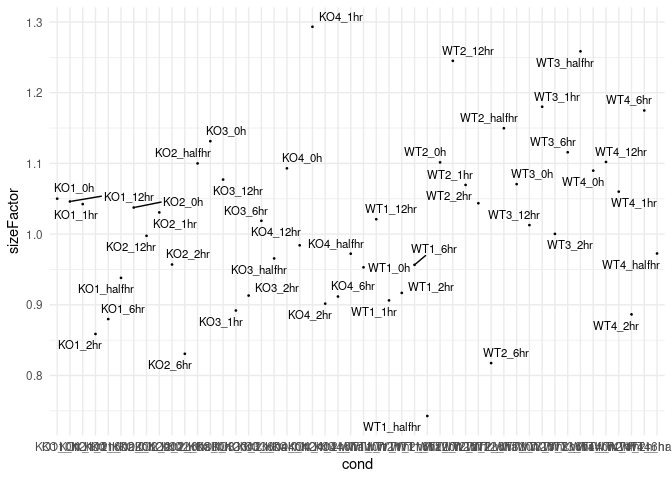
\includegraphics{castor_gao_exp_mk_files/figure-latex/unnamed-chunk-12-1.pdf}

\end{document}
